\documentclass[10pt, letterpaper]{article}

% Inhaltsverzeichnis für Pakettypen (nur für Übersicht im Header, wird nicht im Dokument angezeigt)
% 1. Seitenlayout und Ränder
% 2. Sprache und Zeichensatz
% 3. Mathematik und Theorem-Umgebungen
% 4. Eigene Makros
% 5. Diagramme und Grafiken
% 6. Tabellen und Aufzählungen
% 7. Inhaltsverzeichnis
% 8. Abschnittsüberschriften
% 9. Abstrakt-Umgebung
% 10. Todos/Notizen
% 11. Rahmen/Box-Umgebungen
% 12. Python-Integration
% 13. Literaturverwaltung
% 14. Hyperlinks
% 15. Absatzeinstellungen
% 16. Umgebungen
% 17. Titel und Autor

% --- 1. Seitenlayout und Ränder ---
\usepackage[margin=3cm]{geometry}

% --- 2. Sprache und Zeichensatz ---
\usepackage[english]{babel}
\usepackage[T1]{fontenc}
\usepackage[utf8]{inputenc}

% --- 3. Mathematik und Theorem-Umgebungen ---
\usepackage{amsmath, amssymb, amsthm}
\usepackage{mathrsfs}
\DeclareMathOperator{\WF}{WF}

% --- 4. Eigene Makros ---
\usepackage{xcolor}
\newcommand{\SKP}{\langle\cdot,\cdot\rangle}
\newcommand{\R}{\mathbb{R}}
\newcommand{\N}{\mathbb{N}}
\newcommand{\Q}{\mathbb{Q}}
\newcommand{\Z}{\mathbb{Z}}
\newcommand{\C}{\mathbb{C}}
\newcommand{\entwurf}[1]{\textcolor{red}{#1}}

% --- 5. Diagramme und Grafiken ---
\usepackage{graphicx}
\graphicspath{{../../Images/}}
\usepackage[export]{adjustbox}
\usepackage{tikz}
\usetikzlibrary{decorations.pathreplacing, arrows.meta, positioning}
\usepackage{tikz-cd}

% --- 6. Tabellen und Aufzählungen ---
\usepackage{enumitem}
\setlist[itemize]{left=0.5cm}

\newenvironment{romanenum}[1][]
  {%
    \ifx&#1&
    \else
      \textbf{#1}\quad
    \fi
    \begin{enumerate}[label=\roman*)]
  }
  {%
    \end{enumerate}%
  }

% --- 7. Inhaltsverzeichnis ---
\usepackage{tocloft}
\renewcommand{\cftsecfont}{\footnotesize}
\renewcommand{\cftsubsecfont}{\footnotesize}
\renewcommand{\cftsubsubsecfont}{\footnotesize}
\renewcommand{\cftsecpagefont}{\footnotesize}
\renewcommand{\cftsubsecpagefont}{\footnotesize}
\renewcommand{\cftsubsubsecpagefont}{\footnotesize}
\usepackage{etoc}

% --- 8. Abschnittsüberschriften ---
\usepackage{titlesec}
\titleformat{\section}{\normalfont\large\bfseries}{\thesection}{1em}{}
\titleformat{\subsection}{\normalfont\normalsize\bfseries}{\thesubsection}{0.5em}{}
\titleformat{\subsubsection}{\normalfont\normalsize\bfseries}{\thesubsubsection}{0.5em}{}
\setcounter{secnumdepth}{4}

% --- 9. Abstrakt-Umgebung ---
\usepackage{changepage}
\renewenvironment{abstract}
  {
    \begin{adjustwidth}{1.5cm}{1.5cm}
    \small
    \textsc{Abstract. –}%
  }
  {
    \end{adjustwidth}
  }

% --- 10. Todos/Notizen ---
\usepackage{todonotes}

% --- 11. Rahmen/Box-Umgebungen ---
\usepackage{mdframed}
\usepackage{tcolorbox}
\colorlet{shadecolor}{gray!25}

\newenvironment{customTheorem}
  {\vspace{10pt}%
   \begin{mdframed}[
     backgroundcolor=gray!20,
     linewidth=0pt,
     innertopmargin=10pt,
     innerbottommargin=10pt,
     skipabove=\dimexpr\topsep+\ht\strutbox\relax,
     skipbelow=\topsep,
   ]}
  {\end{mdframed}
   \vspace{10pt}%
  }

% --- 12. Python-Integration ---
% (Deaktiviert in dieser Version, aktiviere bei Bedarf)
% \usepackage{pythontex}
% \usepackage[makestderr]{pythontex}

% --- 13. Literaturverwaltung ---
\usepackage{csquotes}
\usepackage[backend=biber, style=alphabetic, citestyle=alphabetic]{biblatex}
\addbibresource{bibliography.bib}

% --- 14. Hyperlinks ---
\usepackage{hyperref}
\hypersetup{
  colorlinks   = true,
  urlcolor     = blue,
  linkcolor    = blue,
  citecolor    = blue,
  frenchlinks  = true
}

% --- 15. Absatzeinstellungen ---
\usepackage[parfill]{parskip}
\sloppy

% --- 16. Umgebungen ---
\usepackage{thmtools}

\newcommand{\CustomHeading}[3]{%
  \par\medskip\noindent%
  \textbf{#1 #2} \textnormal{(#3)}.\enskip%
}

\newenvironment{DEF}[2]{\CustomHeading{Definition}{#1}{#2}}{}
\newenvironment{PROP}[2]{\CustomHeading{Proposition}{#1}{#2}}{}
\newenvironment{THEO}[2]{\CustomHeading{Theorem}{#1}{#2}}{}
\newenvironment{LEM}[2]{\CustomHeading{Lemma}{#1}{#2}}{}
\newenvironment{KORO}[2]{\CustomHeading{Corollar}{#1}{#2}}{}
\newenvironment{REM}[2]{\CustomHeading{Remark}{#1}{#2}}{}
\newenvironment{EXA}[2]{\CustomHeading{Example}{#1}{#2}}{}
\newenvironment{STUD}[2]{\CustomHeading{Study}{#1}{#2}}{}
\newenvironment{CONC}[2]{\CustomHeading{Concept}{#1}{#2}}{}
\newenvironment{OTH}[2]{\CustomHeading{Other}{#1}{#2}}{}
\newenvironment{EXE}[2]{\CustomHeading{Exercise}{#1}{#2}}{}
\newenvironment{MOT}[2]{\CustomHeading{Motivation}{#1}{#2}}{}
\newenvironment{PROOF}[2]{\CustomHeading{Proof}{#1}{#2}}{}



% --- Unit Umgebung ---
\usepackage{mdframed}
\newmdenv[
  linewidth=1pt,
  topline=false,
  bottomline=false,
  rightline=false,
  leftmargin=0cm,
  rightmargin=0cm,
  skipabove=10pt,
  skipbelow=10pt,
  innertopmargin=0.5\baselineskip,
  innerbottommargin=0.5\baselineskip,
  backgroundcolor=gray!10,
  linecolor=gray
]{unitbox}

\newenvironment{unit}[1]
  {\begin{unitbox}\textbf{Unit #1}\par\smallskip}
  {\end{unitbox}}


% --- 17. Titel und Autor ---
\title{Mein Titel}
\author{Tim Jaschik}
\date{\today}

\begin{document}

\maketitle
\rule{\textwidth}{0.5pt}
\begin{abstract}
Kurze Beschreibung …
\end{abstract}
\rule{\textwidth}{0.5pt}
\vspace{0.5cm}

\tableofcontents

\pagebreak

\section{Knoteninvariante und Knotengruppe}

\subsection{}

\begin{DEF}{KNO-B14-02-33}{Komplement des Knoten}
$V=V(\mathfrak{k})$ denotes a tubular neighborhood of the knot $\mathfrak{k}$ and $C=\overline{S^{3}-V}$ is called the complement of the knot. $H_{j}$ will denote the (singular) homology with coefficients in $\mathbb{Z}$.
\end{DEF}

\begin{THEO}{KNO-S92-01-11}{Glatte Knoten haben tabulare Umgebungen}
A smooth knot $K$ has a tubular neighborhood. That is, there is a neighborhood $\eta(K)$ of $K$ so that the pair $(\eta(K) ; K)$ is diffeomorphic to $S^{1} \times\left(D^{2}, 0\right)$.
\end{THEO}

\begin{DEF}{KNO-B14-03-14}{Alexandroff Kompaktifizierung}
Sei $(X, \mathcal{T})$ ein topologischer Raum und $\infty$ ein Element, das nicht aus $X$ stammt. Zudem sei die Menge $X^*:=X \cup\{\infty\}$ mit der Topologie
$$
\mathcal{T}^*:=\mathcal{T} \cup\left\{X^* \backslash A \mid A \subseteq X, A \text { ist abgeschlossen und kompakt in }(X, \mathcal{T})\right\}
$$
ausgestattet. Dann ist $\left(X^*, \mathcal{T}^*\right)$ ein kompakter Raum, $\operatorname{der}(X, \mathcal{T})=\left(X, \mathcal{T}_{X^*}^*\right)$ als offenen Teilraum enthält. Die Kompaktifizierung ist durch die kanonische Injektion
$$
\iota: X \rightarrow X^*, \quad \iota(x):=x
$$
gegeben. ${ }^{[3]}$ Oft nennt man anstelle von $\iota$ auch den Raum $\left(X^*, \mathcal{T}^*\right)$ die Alexandroff-Kompaktifizierung von $(X, \mathcal{T})$, vorausgesetzt es handelt sich bei $X$ um eine dichte Teilmenge von $X^*$.
Der Punkt $\infty$ wird zuweilen auch als unendlich fern bezeichnet.
\end{DEF}

\begin{DEF}{AT-H09-04-07}{Homotopieäquivalenz zwischen topologischen Räumen}
Eine stetige Abbildung $f: X \rightarrow$ $Y$ wird Homotopieäquivalenz genannt, falls eine stetige Abbildung $g: Y \rightarrow X$ existiert, sodass $g \circ f \simeq \operatorname{id}_{X}$ und $f \circ g \simeq \operatorname{id}_{Y}$ gilt. 

Zwei topologische Räume $X$ und $Y$ heißen homotopieäquivalent, falls eine Homotopieäquivalenz $f: X \rightarrow Y$ existiert. In diesem Fall schreiben wir $X \simeq Y$, und sagen auch $X$ und $Y$ haben denselben Homotopietyp.
\end{DEF}

\begin{DEF}{AT-H09-04-19}{Deformationsretrakte in topologischen Räumen}
Ein Teilraum $A$ eines topologischen Raumes $X$ heißt Deformationsretrakt von $X$ falls eine Homotopie $H$ : $X \times I \rightarrow X$ mit folgenden Eigenschaften existiert:
\begin{enumerate}
\item Eine stetige Abbildung \( H: X \times I \rightarrow X \) mit
\[
H_0 = \operatorname{id}_X, \quad H_1(X) \subseteq A, \quad \text{und} \quad H_t|_A = \operatorname{id}_A \ \text{für alle } t \in I
\]
wird eine \emph{Deformation von \( X \) auf \( A \)} genannt.

\item Die Abbildung \( r := H_1: X \rightarrow A \) heißt dann \emph{Deformationsretraktion}, und \( H \) wird manchmal als \emph{retrahierende Deformation} bezeichnet.

\item Bezeichnet \( \iota: A \rightarrow X \) die kanonische Inklusion, so gilt:
\[
r \circ \iota = \operatorname{id}_A,
\]
d.\,h.\ Deformationsretraktionen sind insbesondere \emph{Retraktionen}.

\item Die Inklusion \( \iota: A \hookrightarrow X \) ist eine \emph{Homotopieäquivalenz}, da
\[
\operatorname{id}_X \simeq \iota \circ r \quad \text{(via \( H \))}.
\]

\item Es wird \emph{nicht} verlangt, dass die Homotopie \( H \) einen Punkt \( x_0 \in A \) festhält, d.\,h.\ es muss nicht gelten, dass
\[
H(x_0, t) = x_0.
\]
\end{enumerate}
\end{DEF}

\begin{EXA}{AT-H09-04-23}{Homotopieäquivalenz zwischen Deformationsretrakt und Ausgangsraum}
Ist $A$ ein Deformationsretrakt von $X$ und $x_{0} \in A$, dann ist die kanonische Inklusion $\left(A, x_{0}\right) \rightarrow\left(X, x_{0}\right)$ eine Homotopieäquivalenz punktierter Räume.
\end{EXA}

\begin{PROP}{AT-H09-03-27}{Induzierter G-Homomorphismus zwischen Fundamentalgruppen für Inklusion von WZSH-Komponente sind Isomorph}
Es sei ( $X, x_{0}$ ) ein punktierter Raum und es bezeichne $X_{0}$ die Wegzusammenhangskomponente von $x_{0}$. Dann induzierte die kanonische Inklusion $\left(X_{0}, x_{0}\right) \rightarrow\left(X, x_{0}\right)$ einen Isomorphismus $\pi_{1}\left(X_{0}, x_{0}\right) \cong \pi_{1}\left(X, x_{0}\right)$.
\end{PROP}

\begin{KORO}{AT-H09-05-05}{Homotopieäquivalente Abbildungen (von Raumpaaren) induzieren isomorphe Homologieabbildungen}
Jede Homotopieäquivalenz von Paaren $f:(X, A) \xrightarrow{\simeq}$ $(Y, B)$ induziert einen Isomorphismus $f_*: H_*(X, A) \stackrel{\cong}{\rightarrow} H_*(Y, B)$ Homotopieäquivalente Paare haben daher isomorphe Homologiegruppen. 

Ebenso induziert eine Homotopieäquivalenz $f: X \xrightarrow{\simeq} Y$ Isomorphismen $f_*: H_*(X) \xrightarrow{\cong} H_*(Y)$ und $f_*: \tilde{H}_*(X) \stackrel{\cong}{\rightarrow} \tilde{H}_*(Y)$. Insbesondere haben homotopieäquivalente Räume isomorphe (reduzierte) Homologiegruppen.
\end{KORO}

\section{Wirtinger Darstellung der Knotengruppe}

\subsection{Freie Gruppen und Darstellungstheorie}

\begin{PROP}{AT-H09-01-01}{Freies Produkt von Gruppen und reduzierte Normalform}
Es seien $G_\alpha$ Gruppen, $\alpha \in A$. Dann existiert eine Gruppe, die wir mit $*_{\alpha \in A} G_\alpha$ bezeichnen und das freie Produkt der $G_\alpha$ nennen, sowie Homomorphismen $\iota_\alpha: G_\alpha \rightarrow *_{\alpha^{\prime} \in A} G_{\alpha^{\prime}}, \alpha \in A$, mit folgenden Eigenschaften:
\begin{enumerate}
  \item $\iota_\alpha$ ist injektiv, wir können daher jede der Gruppen $G_\alpha$ als Untergruppe von $*_{\alpha \in A} G_\alpha$ auffassen und werden die Inklusionen $\iota_\alpha$ meist unterdrücken.
  
  \item $\bigcup_{\alpha \in A} G_\alpha$ erzeugt die Gruppe $*_{\alpha \in A} G_\alpha$. Jedes Element $x \neq 1 \in *_{\alpha \in A} G_\alpha$ lässt sich daher in der Form $x = g_1 \cdots g_n$ mit $g_i \in G_{\alpha_i}$ schreiben. Dabei können wir auch erreichen, dass $g_i \neq 1 \in G_{\alpha_i}$ und $\alpha_i \neq \alpha_{i+1}$ für $i = 1, \ldots, n-1$. Eine solche Darstellung von $x$ wird \emph{reduzierte Darstellung} genannt.
  
  \item Die reduzierte Darstellung von $x \neq 1 \in *_{\alpha \in A} G_\alpha$ ist eindeutig, d.\,h. gilt $g_1 \cdots g_n = x = h_1 \cdots h_m$ und sind beide Darstellungen reduziert, $g_i \in G_{\alpha_i}, h_j \in G_{\beta_j}$, dann folgt $n = m$, $\alpha_i = \beta_i$ und $g_i = h_i$ für alle $i = 1, \ldots, n$.
  
  \item Sind $\varphi_\alpha: G_\alpha \rightarrow K$ Gruppenhomomorphismen, $\alpha \in A$, dann existiert genau ein Gruppenhomomorphismus $\varphi: *_{\alpha \in A} G_\alpha \rightarrow K$, sodass $\varphi \circ \iota_\alpha = \varphi_\alpha$ für alle $\alpha \in A$. Wir werden diesen Homomorphismus mit $*_{\alpha \in A} \varphi_\alpha := \varphi$ bezeichnen.
\end{enumerate}
\end{PROP}

\begin{PROOF}{AT-H09-01-02}{Freies Produkt von Gruppen und reduzierte Normalform}
Unter einem Wort verstehen wir jede endliche Folge $\left(g_1, g_2, \ldots, g_n\right)$ wobei jedes der $g_i$ in einer der Gruppen $G_{\alpha_i}$ liegt. Auch die Folge der Länge 0 ist zugelassen und wird als das leere Wort bezeichnet. Ein Wort $\left(g_1, \ldots, g_n\right)$ heißt reduziert, falls $g_i \neq 1 \in G_{\alpha_i}, i=1, \ldots, n$, und $\alpha_i \neq \alpha_{i+1}$ für $i=1, \ldots, n-1$. Insbesondere ist das leere Wort () reduziert. Es bezeichne $W$ die Menge aller reduzierten Worte, und $\mathfrak{S}(W)$ die Permutationsgruppe von $W$, dh. die Menge der Bijektionen $W \rightarrow W$. Für $\alpha \in A$ und $g \in G_\alpha$ definieren wir eine Abbildung $L_g: W \rightarrow W$ indem wir einem reduzierten Wort $\left(g_1, \ldots, g_n\right)$ mit $g_i \in G_{\alpha_i}$ ein Element in $W$ wie folgt zuordnen:
$$
L_g\left(g_1, \ldots, g_n\right):= \begin{cases}\left(g_1, \ldots, g_n\right) & \text { falls } g=1 \\ \left(g, g_1, \ldots, g_n\right) & \text { falls } g \neq 1 \text { und } \alpha_1 \neq \alpha \\ \left(g g_1, g_2, \ldots, g_n\right) & \text { falls } g \neq 1, \alpha_1=\alpha \text { und } g g_1 \neq 1 \\ \left(g_2, g_3, \ldots, g_n\right) & \text { falls } g \neq 1, \alpha_1=\alpha \text { und } g g_1=1\end{cases}
$$
Eine einfache Fallunterscheidung zeigt $L_1=\operatorname{id}_W$ und $L_h \circ L_g=L_{h g}$ für alle $g, h \in$ $G_\alpha$. Insbesondere ist $L_{g^{-1}}=\left(L_g\right)^{-1}$, jedes $L_g$ daher bijektiv. Wir erhalten einen Gruppenhomomorphismus $\iota_\alpha: G_\alpha \rightarrow \mathfrak{S}(W), g \mapsto L_g$. Wenden wir $L_g$ auf das leere Wort ()$\in W$ an, erhalten wir $L_g(())=(g)$, falls $g \neq 1$, also ist $\iota_\alpha$ injektiv. 

Definieren wir nun $*_{\alpha \in A} G_\alpha$ als die von $\bigcup_{\alpha \in A} \iota_\alpha\left(G_\alpha\right)$ erzeugte Untergruppe in $\mathfrak{S}(W)$, dann sind die Behauptungen (i) und (ii) offensichtlich wahr. 

Nun zu (iii): Sei also $g_1 \cdots g_n=h_1 \cdots h_m \in *_{\alpha \in A} G_\alpha$ mit $g_i \in G_{\alpha_i}$ und $h_j \in G_{\beta_j}$, und so, dass beide Darstellungen reduziert sind. Nach Konstruktion ist $L_{g_1} \circ \cdots \circ L_{g_n}=$ $L_{h_1} \circ \cdots \circ L_{h_m} \in \mathfrak{S}(W)$. Wenden wir diese Permuatation auf das leere Wort () $\in W$ an, dann erhalten wir wegen der Reduziertheit der Darstellungen
$$
\left(g_1, \ldots, g_n\right)=\left(L_{g_1} \circ \cdots \circ L_{g_n}\right)(())=\left(L_{h_1} \circ \cdots \circ L_{h_m}\right)(())=\left(h_1, \ldots, h_m\right),
$$
und damit $n=m, \alpha_i=\beta_i$ sowie $g_i=h_i, i=1 \ldots, n$. 

Nun zu (iv): Seien also Homomorphismen $\varphi_\alpha: G_\alpha \rightarrow K$ gegeben, $\alpha \in A$. Ist $x \neq 1 \in *_{\alpha \in A} G_\alpha$ und $x=g_1 \cdots g_n$ seine reduzierte Darstellung, $g_i \in G_{\alpha_i}$, so definieren wir $\varphi(x):=$ $\iota_{\alpha_1}\left(g_1\right) \cdots \iota_{\alpha_n}\left(g_n\right)$. Setzen wir noch $\varphi(1):=1$, dann liefert dies nach (iii) eine wohldefinierte Abbildung $\varphi: *_{\alpha \in A} G_\alpha \rightarrow K$ für die offensichtlich $\varphi \circ \iota_\alpha=\varphi_\alpha$ gilt, $\alpha \in A$. 

Es bleibt noch zu zeigen, dass $\varphi$ ein Gruppenhomomorphismus ist. Wir zeigen zunächst
$$
\varphi\left(g_1 \cdots g_n\right)=\varphi_{\alpha_1}\left(g_1\right) \cdots \varphi_{\alpha_n}\left(g_n\right), \quad \text { für beliebige } g_i \in G_{\alpha_i} .
$$
Wir werden (I.7) mittels Induktion nach $n$ beweisen. Existiert ein $i$ mit $1 \leq$ $i \leq n$ und $g_i=1 \in G_{\alpha_i}$, dann erhalten wir aus $\varphi_{\alpha_i}\left(g_i\right)=1$ und der Induktionsvoraussetzung $\varphi\left(g_1 \cdots g_n\right)=\varphi\left(g_1 \cdots \hat{i} \cdots g_n\right)=\varphi_{\alpha_1}\left(g_1\right) \cdots \hat{i} \cdots \varphi_{\alpha_n}\left(g_n\right)=$ $\varphi_{\alpha_1}\left(g_1\right) \cdots 1 \cdots \varphi_{\alpha_n}\left(g_n\right)=\varphi_{\alpha_1}\left(g_1\right) \cdots \varphi_{\alpha_i}\left(g_i\right) \cdots \varphi_{\alpha_n}\left(g_n\right)$. Existiert ein $i$ mit $1 \leq$ $i<n$ und $\alpha_i=\alpha_{i+1}$, so folgt aus $\varphi_{\alpha_i}\left(g_i g_{i+1}\right)=\varphi_{\alpha_i}\left(g_i\right) \varphi_{\alpha_{i+1}}\left(g_{i+1}\right)$ und der Induktionsvoraussetzung $\varphi\left(g_1 \cdots g_i g_{i+1} \cdots g_n\right)=\varphi_{\alpha_1}\left(g_1\right) \cdots \varphi_{\alpha_i}\left(g_i g_{i+1}\right) \cdots \varphi_{\alpha_n}\left(g_n\right)=$ $\varphi_{\alpha_1}\left(g_1\right) \cdots \varphi_{\alpha_i}\left(g_i\right) \varphi_{\alpha_{i+1}}\left(g_{i+1}\right) \cdots \varphi_{\alpha_n}\left(g_n\right)$. Tritt keiner der beiden Fälle ein, dann war die Darstellung $g_1 \cdots g_n$ schon reduziert, und es bleibt nichts zu zeigen. 

Damit ist (I.7) bewiesen, woraus wir nun sofort die Homomorphismus Eigenschaft von $\varphi$ erhalten. 

Die Eindeutigkeit von $\varphi$ folgt aus (ii), denn $\varphi$ ist auf einer die Gruppe erzeugenden Teilmenge durch die $\varphi_\alpha$ vorgegeben.
\end{PROOF}

\begin{DEF}{AT-H09-01-03}{Wort und reduzierte Darstellung in freien Gruppen}
Sei $(G_\alpha)_{\alpha \in A}$ eine Familie von Gruppen.
\begin{enumerate}
  \item Ein \emph{(formales) Wort} ist eine endliche Folge $(g_1, \dots, g_n)$, wobei jedes $g_i \in G_{\alpha_i}$ für ein $\alpha_i \in A$ ist. Auch das leere Wort $()$ (d.\,h. die Folge der Länge 0) ist erlaubt.
  
  \item Ein Wort $(g_1, \dots, g_n)$ heißt \emph{reduziert}, wenn
  \begin{itemize}
    \item $g_i \neq 1$ für alle $i = 1, \dots, n$, und
    \item $\alpha_i \neq \alpha_{i+1}$ für alle $i = 1, \dots, n-1$.
  \end{itemize}
  
  \item Die Menge aller reduzierten Worte bezeichnen wir mit $W$.
\end{enumerate}
\end{DEF}

\begin{REM}{AT-H09-01-04}{Permutation des reduzierten Wortes}
Für jedes $\alpha \in A$ und jedes $g \in G_\alpha$ definieren wir eine Abbildung $L_g: W \to W$, die ein reduziertes Wort $(g_1, \dots, g_n)$ gemäß folgender Fallunterscheidung verändert:
\[
L_g(g_1, \dots, g_n) :=
\begin{cases}
(g_1, \dots, g_n) & \text{falls } g = 1 \\
(g, g_1, \dots, g_n) & \text{falls } g \neq 1,\, \alpha \neq \alpha_1 \\
(gg_1, g_2, \dots, g_n) & \text{falls } g \neq 1,\, \alpha = \alpha_1,\, gg_1 \neq 1 \\
(g_2, \dots, g_n) & \text{falls } g \neq 1,\, \alpha = \alpha_1,\, gg_1 = 1
\end{cases}
\]

Die Abbildungen $L_g$ sind bijektiv und erfüllen die Gruppenrelationen:
\[
L_1 = \operatorname{id}_W, \quad L_h \circ L_g = L_{hg}, \quad L_{g^{-1}} = (L_g)^{-1}
\]

Dies definiert einen Gruppenhomomorphismus:
\[
\iota_\alpha: G_\alpha \rightarrow \mathfrak{S}(W), \quad g \mapsto L_g
\]

Wir identifizieren $G_\alpha$ über $\iota_\alpha$ mit seiner injektiven Bildgruppe innerhalb der symmetrischen Gruppe $\mathfrak{S}(W)$.
\end{REM}

\begin{DEF}{AT-H09-01-12}{Freigruppe über einer Menge}
Sei $S$ eine Menge. Dann bezeichnet
\[
F(S) := *_{s \in S} \mathbb{Z}
\]
die \emph{freie Gruppe über $S$}. Es gelten die folgenden Eigenschaften:

\begin{enumerate}[label=(\roman*)]
  \item \textbf{Kanonische Injektionen:}  
  Zu jedem $s \in S$ existiert ein kanonischer injektiver Gruppenhomomorphismus
  \[
  \iota_s : \mathbb{Z} \rightarrow F(S),
  \]
  dessen Bild von $1 \in \mathbb{Z}$ wir mit $s$ bezeichnen, also $\iota_s(1) = s$.

  \item \textbf{Wortdarstellung:}  
  Jedes Element $x \in F(S) \setminus \{1\}$ lässt sich eindeutig schreiben als
  \[
  x = s_1^{k_1} s_2^{k_2} \cdots s_n^{k_n},
  \]
  wobei $s_i \in S$, $k_i \in \mathbb{Z} \setminus \{0\}$ und $s_i \neq s_{i+1}$ für alle $i = 1, \dots, n-1$.

  \item \textbf{Universelle Eigenschaft:}  
  Ist $K$ eine Gruppe und für jedes $s \in S$ ein Element $k_s \in K$ gegeben, so existiert ein eindeutig bestimmter Gruppenhomomorphismus
  \[
  \varphi : F(S) \longrightarrow K
  \]
  mit $\varphi(s) = k_s$ für alle $s \in S$.
\end{enumerate}
\end{DEF}

\begin{DEF}{AT-H09-01-13}{Freie Gruppen von Rang $k$}
Eine Gruppe $G$ heißt frei falls eine Menge $S$ existiert, sodass $G \cong F(S)$. Die Kardinalzahl $\sharp S$ wird der Rang der freien Gruppe $G$ genannt und mit $\operatorname{rank}(G)$ bezeichnet. Dies ist wohldefiniert, denn aus $F(S) \cong F\left(S^{\prime}\right)$ folgt $\bigoplus_{s \in S} \mathbb{Z} \cong F(S)^{\text {ab }} \cong$ $F\left(S^{\prime}\right)^{\mathrm{ab}} \cong \bigoplus_{s^{\prime} \in S^{\prime}} \mathbb{Z}$ und damit $\sharp S=\sharp S^{\prime}$.
\end{DEF}

\begin{CONC}{AT-H09-01-14}{Freie Gruppen modulo erzeugter Normalteiler einer Teilmenge der freien Gruppe über Menge }
Ist $R \subseteq F(S)$ eine Teilmenge so schreiben wir 
$$\langle S \mid R\rangle:=F(S) / \mathcal{N}(R)$$ 
wobei $\mathcal{N}(R)$ den von $R$ erzeugten Normalteiler in $F(S)$ bezeichnet.
\end{CONC}

\begin{DEF}{AT-H09-01-15}{Darstellung einer Gruppe durch Erzeuger und Relationen}
Ist $G$ eine Gruppe und $G \cong\langle S \mid R\rangle$ dann nennen wir $\langle S \mid R\rangle$ eine Präsentation von $G$ mit Erzeugern $S$ und Relationen $R$.
\end{DEF}

\begin{DEF}{AT-H09-01-17}{Endlich repräsentierbare Gruppe}
Eine Gruppe $G$ wird endlich präsentierbar, geannt, falls eine Präsentation $G \cong\langle S \mid R\rangle$ mit endlichen Mengen $S$ und $R$ existiert. Ist $S=\left\{s_1, \ldots, s_n\right\}$ und $R=\left\{r_1, \ldots, r_m\right\}$ dann schreiben wir für $\langle S \mid R\rangle$ auch $\left\langle s_1, \ldots, s_n \mid r_1, \ldots, r_m\right\rangle$ oder $\left\langle s_1, \ldots, s_n \mid r_1=1, \ldots, r_m=1\right\rangle$.
\end{DEF}

\begin{PROP}{AT-H09-01-16}{Universelle Eigenschaft der Darstellung einer Gruppe}
Sei nun $K$ eine weitere Gruppe und für jedes $s \in S$ ein $k_s \in K$ gegeben, sodass der durch $\tilde{\varphi}(s)=k_s$ bestimmte Homomorphismus $\tilde{\varphi}$ : $F(S) \rightarrow K$ auf jedem Element von $R$ verschwindet, dh. $\tilde{\varphi}(r)=1 \in K$ für alle $r \in R$. Dann ist $\mathcal{N}(R) \subseteq \operatorname{ker}(\tilde{\varphi})$, also faktorisiert $\tilde{\varphi}$ zu einem Homomorphismus 
$$\varphi:\langle R \mid S\rangle=F(S) / \mathcal{N}(R) \rightarrow K$$ 
mit $\varphi(s)=k_s$.
\end{PROP}

\begin{LEM}{AT-H09-01-18}{Präsentation jeder Gruppe}
Jede Gruppe $G$ besitzt die Präsentation
\[
G=\langle S \mid R\rangle \quad\text{mit } S := G,\; R := \ker(\varphi),
\]
wobei $\varphi: F(S) \rightarrow G$ der durch $\varphi(g)=g$ gegebene Homomorphismus ist.
Es faktorisiert dann $\varphi$ zu einem (offensichtlich bijektiven) Homomorphismus
\[
\langle S \mid R\rangle = F(S)/\mathcal{N}(R) = F(S)/\ker(\varphi) \longrightarrow G.
\]
\end{LEM}

\begin{LEM}{AT-H09-01-19}{Hinzufügen von überflüssigen Relationen}
Ist $r \in \mathcal{N}(R)$, dann gilt
\[
\mathcal{N}(R) = \mathcal{N}(R \cup \{r\}),
\quad\text{und daher}\quad
\langle S \mid R \rangle \cong \langle S \mid R \cup \{r\} \rangle.
\]
\end{LEM}

\begin{LEM}{AT-H09-01-20}{Einführen eines neuen Erzeugers}
Ist $t \notin S$ und $\omega \in F(S)$, dann gilt
\[
\langle S \mid R\rangle \cong \left\langle S \cup \{t\} \mid R \cup \{t^{-1} \omega\} \right\rangle.
\]
\end{LEM}

\begin{PROOF}{AT-H09-01-21}{P: Einführen eines neuen Erzeugers}
Zum Nachweis der Isomorphie sei
\[
\varphi: \langle S \mid R\rangle \to \left\langle S \cup \{t\} \mid R \cup \{t^{-1}\omega\} \right\rangle
\]
der durch $\varphi(s) = s$ für $s \in S$ eindeutig bestimmte Homomorphismus.

Weiters sei
\[
\psi: \left\langle S \cup \{t\} \mid R \cup \{t^{-1}\omega\} \right\rangle \to \langle S \mid R\rangle
\]
definiert durch $\psi(s) = s$ für $s \in S$, sowie $\psi(t) = \omega$.

Dann gilt: $\psi \circ \varphi = \mathrm{id}$ und $\varphi \circ \psi = \mathrm{id}$, denn
\[
\varphi(\psi(t)) = \varphi(\omega) = t.
\]
\end{PROOF}

\begin{DEF}{AT-H09-01-22}{Tietze-Transformationen}
Sind $\langle S \mid R\rangle$ und $\langle S' \mid R'\rangle$ zwei endliche Präsentationen derselben Gruppe, also
\[
\langle S \mid R\rangle \cong \langle S' \mid R'\rangle,
\]
so lässt sich jede Präsentation durch endlich viele Schritte der Art
$$
\langle S \mid R\rangle \cong\langle S \mid R \cup\{r\}\rangle .
$$
und
$$
\langle S \mid R\rangle \cong\left\langle S \cup\{t\} \mid R \cup\left\{t^{-1} \omega\right\}\right\rangle .
$$
(Tietze-Prozesse) ineinander überführen.
\end{DEF}

\begin{LEM}{AT-H09-01-24}{Abelsierung von präsentierten Gruppen durch Kommutatoren}
Die Abelsierung einer präsentierten Gruppe ergibt sich durch Hinzufügen der Kommutatorrelationen:
\[
\langle S \mid R\rangle^{\mathrm{ab}} \cong \langle S \mid R \cup K\rangle,
\]
wobei $K = \{ sts^{-1}t^{-1} \mid s \neq t \in S \}$.

Der durch $\tilde{\varphi}(s) = s$ definierte Homomorphismus
\[
\tilde{\varphi}: \langle S \mid R\rangle \to \langle S \mid R \cup K\rangle
\]
faktorisiert zu einem Isomorphismus
\[
\varphi: \langle S \mid R\rangle^{\mathrm{ab}} \to \langle S \mid R \cup K\rangle,
\]
invers zum Homomorphismus $\psi(s) = s$, mit $\varphi \circ \psi = \mathrm{id}$ und $\psi \circ \varphi = \mathrm{id}$.
\end{LEM}

\begin{EXA}{AT-H09-01-25}{Präsentation von Gruppen}
Für $n \in \mathbb{Z}$ schreiben wir $\mathbb{Z}_n:=\mathbb{Z} / n \mathbb{Z}$. Dies eine endliche zyklische Gruppe falls $n \neq 0$.
\begin{enumerate}[label=(\roman*)]
  \item $\langle s \mid - \rangle \;\cong\; \mathbb{Z}.$
  \item $\langle s, t \mid - \rangle \;\cong\; \mathbb{Z} * \mathbb{Z}.$
  \item $\langle s, t \mid s t s^{-1} t^{-1} \rangle \;\cong\; \mathbb{Z} \oplus \mathbb{Z}.$
  \item $\langle s \mid s^{n} \rangle \;\cong\; \mathbb{Z}_{n}, \quad n \in \mathbb{Z}.$
  \item $\langle s, t \mid s^{m},\, t^{n} \rangle \;\cong\; \mathbb{Z}_{m} * \mathbb{Z}_{n}, \quad m,n \in \mathbb{Z}.$
  \item $\langle s, t \mid s^{m},\, t^{n},\, s t s^{-1} t^{-1} \rangle 
        \;\cong\; \mathbb{Z}_{m} \oplus \mathbb{Z}_{n}, \quad m,n \in \mathbb{Z}.$
  \item $\langle s, t \mid s^{2} t^{3},\, s^{3} t^{4} \rangle \;=\; 0.$
\end{enumerate}
\end{EXA}

\subsection{Wirtinger Theorem}

\begin{THEO}{KNO-B14-03-01}{Wirtinger Presentation}
Let $\sigma_{i}, i=1,2, \ldots, n$, be the overcrossing arcs of a regular projection of a knot (or link) $\mathfrak{k}$. Then the knot group admits the following so-called Wirtinger presentation:
$$
\mathfrak{G}=\pi_{1}\left(\overline{S^{3}-V(\mathfrak{f})}\right)=\left\langle s_{1}, \ldots, s_{n} \mid r_{1}, \ldots, r_{n}\right\rangle .
$$
The arc $\sigma_{i}$ corresponds to the generator $s_{i}$; a crossing of characteristic $\eta_{j}$ as in Figure 3.2 gives rise to the defining relations
$$
r_{j}=s_{j} s_{i}^{-\eta_{j}} s_{k}^{-1} s_{i}^{\eta_{j}} .
$$
\end{THEO}

\begin{THEO}{AT-H09-01-30}{Seifert van Kampen}
Es sei $X=U \cup V$ wobei $U$ und $V$ offen in $X$ sind. Weiters seien $U, V$ sowie $U \cap V$ wegzusammenhängend und $x_0 \in$ $U \cap V$. Dann ist die Abbildung
$$\Phi:=\left(\iota_U\right)_* *\left(\iota_V\right)_*: \pi_1\left(U, x_0\right) * \pi_1\left(V, x_0\right) \rightarrow \pi_1\left(X, x_0\right)$$
surjektiv, und es gilt 
$$\operatorname{ker}(\Phi)= N:=\mathcal{N}\left(\left\{\left(\left(j_U\right)_* \sigma\right)\left(\left(j_V\right)_* \sigma\right)^{-1}: \sigma \in \pi_1\left(U \cap V, x_0\right)\right\}\right)$$ 
Insbesondere ist $\pi_1\left(X, x_0\right) \cong\left(\pi_1\left(U, x_0\right) * \pi_1\left(V, x_0\right)\right) / N$.
\end{THEO}

\begin{EXA}{AT-H09-01-29}{Fundamentalgruppen von Einpunktvereinigungen von $S^1$}
Für $n_i \geq 2$ ist $S^{n_1} \vee \cdots \vee S^{n_k}$ einfach zusammenhängend, siehe Satz I.1.26 und Proposition I.5.8. 

Mit Hilfe von Satz I.2.1 erhalten wir aber auch $\pi_1\left(S^1 \vee \cdots \vee S^1\right) \cong \mathbb{Z} * \cdots * \mathbb{Z}$. 

Einpunktvereinigungen von Kreisen können also nur dann homotopieäquivalent (homöomorph) sein, wenn sie gleich viele Faktoren besitzen, siehe Beispiel I.5.3 und Satz I.3.27.
\end{EXA}

\section{Knotengruppe als Invariante}

\subsection{Papakyriakopoulos Theorem}

\begin{PROP}{KNO-B14-03-04}{Fundamentalgruppe des Komplements von tabularen Umgebungen charakterisiert den trivialen Knoten}
If $\mathfrak{k}$ is a non-trivial knot the inclusion $i: \partial V \rightarrow C=\overline{S^{3}-V}$ induces an injective homomorphism $i_{\#}: \pi_{1} \partial V \rightarrow \pi_{1} C$. In particular, if $\pi_{1} C \cong \mathbb{Z}$ is cyclic then the knot $\mathfrak{k}$ is trivial.
\end{PROP}

\begin{PROP}{KNO-B14-04-01}{Homologische Eigenschaften von tabuieren Umgebungen von Knoten}
$V=V(\mathfrak{k})$ denotes a tubular neighborhood of the knot $\mathfrak{k}$ and $C=\overline{S^{3}-V}$ is called the complement of the knot. $H_{j}$ will denote the (singular) homology with coefficients in $\mathbb{Z}$.

\begin{itemize}
  \item[(a)] \( H_{0}(C) \cong H_{1}(C) \cong \mathbb{Z}, \quad H_{n}(C) = 0 \) for \( n \geq 2 \).
  
  \item[(b)] There are two simple closed curves \( m \) and \( \ell \) on \( \partial V \) with the following properties:
  \begin{enumerate}
    \item \( m \) and \( \ell \) intersect in one point,
    \item \( m \sim 0 \), \( \ell \sim \mathfrak{k} \) in \( V(\mathfrak{k}) \),
    \item \( \ell \sim 0 \) in \( C = \overline{S^{3} - V(\mathfrak{k})} \),
    \item \( \operatorname{lk}(m, \mathfrak{k}) = 1 \) and \( \operatorname{lk}(\ell, \mathfrak{k}) = 0 \) in \( S^{3} \).
  \end{enumerate}
\end{itemize}

These properties determine $m$ and $\ell$ up to isotopy on $\partial V(\mathfrak{k})$. We call $m$ a meridian and $\ell$ a longitude of the knot $\mathfrak{k}$. The knot $\mathfrak{k}$ and the longitude $\ell$ bound an annulus $A \subset V$.
\end{PROP}

\begin{PROOF}{KNO-B14-04-02}{P: Homologische Eigenschaften von tabuieren Umgebungen von Knoten}
Consider the isomorphism
$$
\mathbb{Z} \oplus \mathbb{Z} \cong H_{1}(\partial V) \rightarrow H_{1}(V) \oplus H_{1}(C)
$$
in the Mayer-Vietoris sequence. The generators of $H_{1}(V) \cong \mathbb{Z}$ and $H_{1}(C) \cong \mathbb{Z}$ are determined up to their inverses. Choose the homology class of $\mathfrak{k}$ as a generator of $H_{1}(V)$ and represent it by a simple closed curve $\ell$ on $\partial V$ which is homologous to 0 in $H_{1}(C)$. These conditions determine the homology class of $\ell$ in $\partial V$; hence, $\ell$ is unique up to isotopy on $\partial V$. 

A generator of $H_{1}(C)$ can be represented by a curve $m$ on $\partial V$ that is homologous to 0 in $V$. 

The curves $\ell$ and $m$ determine a system of generators of $H_{1}(\partial V) \cong \mathbb{Z} \oplus \mathbb{Z}$. 

By a well-known result, we may assume that $m$ is simple and intersects $\ell$ in one point, see e.g. Stillwell [345, 6.4.3], Zieschang, Vogt and Coldewey [382, E 3.22]. 

As $m$ is homologous to 0 in $V$ it is null-homotopic in $V$, bounds a disk, and is a meridian of the solid torus $V$. 

The linking number of $m$ and $\mathfrak{F}$ is 1 or -1. If necessary we reverse the direction of $m$ to get (4). 

These properties determine $m$ up to an isotopy of $\partial V$. 

A consequence is that $\ell$ and $\mathfrak{k}$ bound an annulus $A \subset V$.

Since $\ell \sim 0$ in $C, \ell$ bounds a surface, possibly with singularities, in $C$. (As we already know, see Proposition 2.4, $\ell$ even spans a surface without singularities: a Seifert surface.)
\end{PROOF}

\begin{THEO}{KNO-B14-02-34}{Papakyriakopoulos Loop Theorem}
Let $M$ be a 3-manifold and let $B$ be a component of its boundary. If there are elements in $\operatorname{ker}\left(\pi_1 B \rightarrow \pi_1 M\right)$ which are not contained in a given normal subgroup $\Re$ of $\pi_1(B)$ then there is a simple loop $C$ on $B$ such that $C$ bounds a non-singular disk in $M$ and $[C] \notin \Re$.
\end{THEO}

\begin{PROOF}{KNO-B14-03-05}{P: Fundamentalgruppe des Komplements von tabularen Umgebungen charakterisiert den trivialen Knoten}
Suppose $i_{\#}$ is not injective. Then the Loop Theorem of Papakyriakopoulos [281], see Appendix B.5 [159, 4.2], guarantees the existence of a simple closed curve $\kappa$ on $\partial V$ and a disk $\delta$ in $C$ such that
$$
\kappa = \partial \delta 
\quad \text{(hence } \kappa \simeq 0 \text{ in } C\text{),} \quad 
\delta \cap V = \kappa \quad \text{and} \quad 
\kappa \not\simeq 0 \text{ in } \partial V\text{.}
$$
Since $\kappa$ is simple and $\kappa \sim 0$ in $C$ it is a longitude, see 3.2. So there is an annulus $A \subset V$ such that $A \cap \partial V=\kappa, \partial A=\kappa \cup \mathfrak{k}$, as has been shown in Theorem 3.1. This proves that $\mathfrak{k}$ bounds a disk in $S^{3}$ and, hence, is the trivial knot.
\end{PROOF}

\begin{REM}{KNO-B14-02-06}{Homeomorphismus zwischen Komplementen der Einbettungen}
The restriction
$$
h_{1} \mid:\left(Y-f_{0}(X)\right) \rightarrow\left(Y-f_{1}(X)\right)
$$
of the homeomorphism $h_{1}: Y \rightarrow Y$ is itself a homeomorphism of the complements of $f_{0}(X)$ resp. $f_{1}(X)$ in $Y$, if $f_{0}$ and $f_{1}$ are ambient isotopic. This is not necessarily true in the case of mere isotopy and marks the crucial difference.
\end{REM}

\begin{REM}{KNO-B14-02-35}{Anmerkungen zum Papakyriakopoulos Loop Theorem}
The Papakyriakopoulos Loop Theorem was proved by Papakyriakopoulos [281] and Stallings [342]. Proofs in books are available, see Rolfsen [309], Hempel [159] and Jaco [176]. See also Hatcher's notes [156].

Remark. The proof is given in the second reference. The original version of the loop theorem ( $\Re=1$ ) was first formulated and proved by Papakyriakopoulos. Another generalization analogous to the Shapiro-Whitehead version of Dehn's Lemma was proved by Waldhausen [364].
\end{REM}

\subsection{Effektivität der Wirtinger Darstellung}

\begin{MOT}{KNO-F12-03-01}{Reichweite der Knotengruppe als Knoten Invariante}
Wir haben jetzt also eine Präsentation für $\pi_1\left(\mathbb{R}^3 \backslash K\right)$ gefunden. Aber was bringt uns das? Wir möchten gerne zeigen, dass $K$ nicht der triviale Knoten $T$ ist, d.h. das $\pi_1\left(\mathbb{R}^3 \backslash K\right) \neq \pi_1\left(\mathbb{R}^3 \backslash T\right)=\mathbb{Z}$. Die Präsentation von $\pi:=\pi_1\left(\mathbb{R}^3 \backslash K\right)$ schaut zwar kompliziert aus, aber vielleicht ist die Gruppe trotz allem isomorph zu $\mathbb{Z}$?
\end{MOT}

\begin{CONC}{KNO-F12-03-04}{Word Problem für Präsentationen von Knotengruppen}
Es sei
$$
\pi=\left\langle g_1, \ldots, g_k \mid r_1, \ldots, r_l\right\rangle
$$
eine Präsentation einer Gruppe. Gibt es einen Algorithmus, welcher entscheiden kann, ob $\pi$ trivial ist oder isomorph zu $\mathbb{Z}$ ist?

Diese Frage ist als das 'word problem' bekannt, und wurde von Adyan und Rabin 1955 beantwort: Sie haben unabhängig von einander bewiesen, dass es solch einen Algorithmus nicht geben kann. Im Allgemeinen können wir also nicht entscheiden, ob eine gegebene Präsentation die Präsentation der trivialen Gruppe ist oder nicht.

Diese negative Aussage raubt uns erstmal alle Hoffnung, dass wir Fundamentalgruppen von Knotenkomplement verwenden können, um festzustellen, ob ein gegebener Knoten trivial ist oder nicht. Zum Glück ist unser Leben aber etwas einfacher: nicht jede Präsentation taucht als Präsentation der Fundamentalgruppe eines Knotenkomplements auf.
\end{CONC}

\begin{THEO}{KNO-F12-03-05}{Thurston 1982}
Es sei $K \subset \mathbb{R}^3$ ein nicht-trivialer Knoten, dann gibt es einen Epimorphismus $\pi_1\left(\mathbb{R}^3 \backslash K\right) \rightarrow G$ auf eine endliche nicht-kommutative Gruppe.
\end{THEO}

\begin{CONC}{KNO-F12-03-06}{Äquivalenz von Knoten bis auf Spiegelung}
Man kann sich nun auch fragen, ob zwei Knoten $K$ und $L$ genau dann äquivalent sind, wenn $\pi_1\left(\mathbb{R}^3 \backslash K\right) \cong \pi_1\left(\mathbb{R}^3 \backslash L\right)$. Dies ist im Allgemeinen jedoch nicht der Fall. Für einen Knoten $K$ bezeichnen wir mit $K^s$ das Spiegelbild von $K$ in der Ebene $(x, y, 0) \subset \mathbb{R}^3$, d.h.
$$
(x, y, z) \in K^s: \Leftrightarrow(x, y,-z) \in K .
$$
Dann sind $\mathbb{R}^3 \backslash K^s$ und $\mathbb{R}^3 \backslash K$ offensichtlich homöomorph, also besitzen sie die gleiche Fundamentalgruppe. Andererseits sind im Allgemeinen ein Knoten und sein Spiegelbild nicht äquivalent.

Wir können also jetzt etwas vorsichtiger fragen ob zwei Knoten $K$ und $L$ genau dann (bis auf Spiegelung) äquivalent sind, wenn $\pi_1\left(\mathbb{R}^3 \right.$ $K) \cong \pi_1\left(\mathbb{R}^3 \backslash L\right)$.

Um diese Frage zu diskutieren brauchen wir den Begriff der zusammenhängenden Summe $K \# L$ von orientierten Knoten $K$ und $L$, welcher in Abbildung 44 eingeführt wird. Wenn $K$ ein orientierter Knoten ist, dann bezeichnen wir mit $\bar{K}$ den gleichen Knoten mit umgekehrter Orientierung. Mithilfe des Satzes von Seifert-van Kampen kann man relativ leicht zeigen, dass für alle orientierten Knoten $K$ und $L$ gilt
$$
\pi_1\left(\mathbb{R}^3 \backslash K \# L\right) \cong \pi_1\left(\mathbb{R}^3 \backslash \bar{K} \# L\right),
$$
andererseits gibt es Knoten $K$ und $L$, so dass $\bar{K} \# L$ weder mit $K \# L$ noch mit dem Spiegelbild von $K \# L$ übereinstimmt.

Wir sagen nun, dass ein Knoten $K$ ein Primknoten ist, wenn $K$ nicht die zusammenhängende Summe von zwei nicht-trivialen Knoten ist. Folgender Satz wurde von Culler-Gordon-Luecke-Shalen-Witten ${ }^{96}$ bewiesen:
\end{CONC}

\begin{THEO}{KNO-F12-03-07}{Culler-Gordon-Luecke-Shalen-Witten 1989}
Es seien $K, J \subset \mathbb{R}^3$ zwei Primknoten mit $\pi_1\left(\mathbb{R}^3 \backslash K\right) \cong \pi_1\left(\mathbb{R}^3 \backslash J\right)$, dann gilt $K=J$ oder $K=J^s$.
\end{THEO}

\begin{CONC}{KNO-B14-03-13}{Settings zur Untersuchung der Knotengruppe}
The most important and effective invariant of a knot $\mathfrak{k}$ (or link) is its group: the fundamental group of its complement $\mathfrak{G}=\pi_{1}\left(S^{3}-\mathfrak{k}\right)$. Frequently $S^{3}-\mathfrak{k}$ is replaced by $\mathbb{R}^{3}-\mathfrak{k}$ or by $\overline{S^{3}-V(\mathfrak{k})}$ or $\overline{\mathbb{R}^{3}-V(\mathfrak{k})}$, respectively. The fundamental groups of these various spaces are obviously isomorphic, the isomorphisms being induced by inclusion.
\end{CONC}

\begin{THEO}{KNO-F12-03-08}{Gordon–Luecke Theorem 1989}
If the complements of two tame knots are homeomorphic, then the knots are equivalent.
\end{THEO}

\subsection{Abelisierte Knotengruppe als Invariante}

\begin{PROP}{AT-H09-02-09}{Hurewicz-Homomorphismus induziert einen Isomorphismus für abelisierte Fundamentalgruppe für WZSH punktierte Räume}
Es sei $(X, x_0)$ ein wegzusammenhängender punktierter Raum. Dann ist der Hurewicz-Homomorphismus 
$$\tilde{h}_n=\tilde{h}_n^X:\left[S^n, X\right] \rightarrow H_n(X), \quad \tilde{h}_n([\sigma]):=\sigma_*\left(\alpha_n\right)$$
surjektiv und sein Kern stimmt mit der Kommutatoruntergruppe von $\pi_1\left(X, x_0\right)$ überein. Er induziert daher einen Isomorphismus $\pi_1\left(X, x_0\right)_{\mathrm{ab}} \cong H_1(X)$.
\end{PROP}

\begin{PROP}{KNO-B14-04-03}{Homologie des Knotenkomplements}
Let \( C = \overline{S^3 \setminus V} \) be the complement of the knot. We consider singular homology with integer coefficients, i.e., \( H_j = H_j(-; \mathbb{Z}) \). Then:
\[
H_j(C) \cong
\begin{cases}
\mathbb{Z} & \text{if } j = 0 \text{ or } j = 1, \\
0 & \text{otherwise}.
\end{cases}
\]
\end{PROP}

\begin{PROOF}{KNO-B14-04-04}{Homologie des Knotenkomplements}
Here we present one based on homological methods. We use the following well-known results:
$$
H_{n}\left(S^{3}\right)= \begin{cases}\mathbb{Z} & \text { for } n=0,3 \\ 0 & \text { otherwise }\end{cases}
$$
$$
\begin{aligned}
H_{n}(\partial V) & = \begin{cases}\mathbb{Z} & \text { for } n=0,2 \\
\mathbb{Z} \oplus \mathbb{Z} & \text { for } n=1, \\
0 & \text { otherwise, }\end{cases} \\
H_{n}(V)=H_{n}\left(S^{1}\right)= & \begin{cases}\mathbb{Z} & \text { for } n=0,1, \\
0 & \text { otherwise; }\end{cases}
\end{aligned}
$$
they can be found in standard books on algebraic topology, see Spanier [341], StöckerZieschang [346], Hatcher [157].

Since $C$ is connected, $H_{0}(C)=\mathbb{Z}$. For further calculations we use the MayerVietoris sequence of the pair ( $V, C$ ) where $V \cup C=S^{3}, V \cap C=\partial V$ :
\[
\begin{tikzcd}[row sep=small, column sep=small]
H_3(\partial V) \arrow[r] \arrow[d, equal] 
  & H_3(V) \arrow[r, phantom, "\oplus"] \arrow[d, equal] 
  & H_3(C) \arrow[r] 
  & H_3(S^3) \arrow[r] \arrow[d, "\cong", "\mathbb{Z}"']
  & H_2(\partial V) \arrow[r] \arrow[d, "\cong", "\mathbb{Z}"'] 
  & {} \\
0 & 0 & {} & \mathbb{Z} & \mathbb{Z} & {}
\end{tikzcd}
\]

\[
\begin{tikzcd}[row sep=small, column sep=small]
{} \arrow[r]
  & H_2(V) \arrow[r, phantom, "\oplus"] \arrow[d, equal]
  & H_2(C) \arrow[r] 
  & H_2(S^3) \arrow[r] \arrow[d, equal]
  & H_1(\partial V) \arrow[r] \arrow[d, "\cong"]
  & {} \\
{} & 0 & {}& 0 & \mathbb{Z} \oplus \mathbb{Z} & {}
\end{tikzcd}
\]

\[
\begin{tikzcd}[row sep=small, column sep=small]
{} \arrow[r] 
  & H_1(V) \arrow[r, phantom, "\oplus"] \arrow[d, "\cong"] & H_1(C) \arrow[r]
  & H_1(S^3) \arrow[d, equal] \\
{} & \mathbb{Z} & {} & 0
\end{tikzcd}
\]
It follows that $H_{1}(C)=\mathbb{Z}$. Since $\partial V$ is the boundary of the orientable compact 3manifold $C$, the group $H_{2}(\partial V)$ is mapped by the inclusion $\partial V \hookrightarrow C$ to $0 \in H_{2}(C)$. This implies that $H_{2}(C)=0$ and that $H_{3}\left(S^{3}\right) \rightarrow H_{2}(\partial V)$ is surjective; hence, $H_{3}(C)=0$.


Since $C$ is a 3-manifold it follows that $H_{n}(C)=0$ for $n>3$; this is also a consequence of the Mayer-Vietoris sequence.
\end{PROOF}

\section{Appendix}

\subsection{Meridian und Longitude}

\begin{DEF}{KNO-S92-01-13}{Rand von tabularen Knoten-Umgebungen sind diffeomorph zu $S^1\times S^1$ (Meridian, Longitude)}
The boundary $\partial \eta(K)$ of a tubular neighborhood of $K$ is diffeomorphic to the torus $S^{1} \times S^{1}$. It contains two special circles:\\
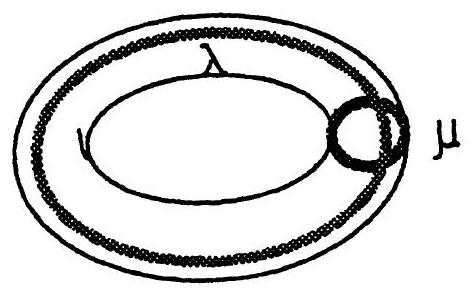
\includegraphics[scale=0.2, center]{2025_05_21_037de704f595ce642d3eg-080}

Fig. 7. Meridian $\mu$ and longitude $\lambda$.

The meridian is the boundary of a cross-sectional disk $\{*\} \times D^{2} \subset S^{1} \times D^{2}$ and is denoted $\mu$.

The longitude is denoted $\lambda$ and is the boundary of a Seifert surface.
\end{DEF}

\begin{THEO}{KNO-S92-01-14}{Meridan und Longitude von Knoten sind eindeutig bis auf Isotopie}
The meridian and longitude of a knot $K$ are uniquely defined in $\partial \eta(K)$ up to isotopy.
\end{THEO}

\begin{PROOF}{KNO-S92-01-15}{P: Meridan und Longitude von Knoten sind eindeutig bis auf Isotopie}
Proof: The harder part is showing the uniqueness of $\lambda$. This can be done by studying the arcs of intersection of two different Seifert surfaces. Alternately, there's an easy proof from algebraic topology. First note that two simple closed curves $c$ and $c^{\prime}$ imbedded in $S^{1} \times S^{1}$ are isotopic if and only if the algebraic intersection $c \cdot c^{\prime}$ is trivial. If $S$ and $S^{\prime}$ are two Seifert surfaces for $K$, then $\partial S \cdot \partial S^{\prime}=\partial\left[S \cdot S^{\prime}\right]$. But $S \cdot S^{\prime}$ is in $H_{1}(M, \partial M)$, which is trivial.
\end{PROOF}

\begin{REM}{KNO-S92-01-16}{Charakterisierung von einfachen geschlossen Kurven im tabularen Rand durch Meridian und Longitude}
The natural choice of circles $\lambda$ and $\mu$ then allows us to describe any simple closed curve on $\partial \eta(K)$ by a number in the extended rationals $Q \cup(\infty)$. The curve homologous to $p \mu+q \lambda$ we associate with the rational number $p / q$. (e. g. $\mu \rightarrow \infty$ ).
\end{REM}

\subsection{Hilfssätze}

\subsection{Hurewicz-Isomorphismus}

\begin{CONC}{AT-H09-02-04}{Herleitung der Hurewicz-Abbildung}
Es sei $n \geq 1$. Nach Satz IV.9.5 ist $H_n\left(S^n\right) \cong \mathbb{Z}$, die Gruppe $H_n\left(S^n\right)$ besitzt daher zwei Erzeuger. Wir fixieren einen dieser Erzeuger $\alpha_n \in H_n\left(S^n\right)$, nämlich den aus Proposition IV.9.9, und bezeichnen ihn von nunan als den Standarderzeuger von $H^n\left(S^n\right)$.

Ist $\sigma: S^n \rightarrow X$ eine stetige Abbildung so erhalten wir eine Homologieklasse $\sigma_*\left(\alpha_n\right) \in H_n(X)$. Nach Korollar IV.7.5 hängt diese Homotopieklasse nur von der Homotopieklasse von $\sigma$ ab, die Konstruktion liefert daher eine wohldefinierte Abbildung
$$
\tilde{h}_n=\tilde{h}_n^X:\left[S^n, X\right] \rightarrow H_n(X), \quad \tilde{h}_n([\sigma]):=\sigma_*\left(\alpha_n\right) .
$$
Diese Abbildung ist natürlich, dh. für jede stetige Abbildung $f: X \rightarrow Y$ kommutiert das Diagramm
\[
\begin{tikzcd}
{[S^n, X]} \arrow[r, "\tilde{h}_n^X"] \arrow[d, "f_*"'] & H_n(X) \arrow[d, "f_*"] \\
{[S^n, Y]} \arrow[r, "\tilde{h}_n^Y"'] & H_n(Y)
\end{tikzcd}
\]
wobei die Abbildung $f_*:\left[S^n, X\right] \rightarrow\left[S^n, Y\right]$ durch $f_*([\sigma])=$ $[f \circ \sigma]$ gegeben ist, vgl. Bemerkung I.3.6. 

Um dies einzusehen betrachten wir eine beliebige stetige Abbildung $\sigma: S^n \rightarrow X$. Aus der Funktorialität der Homologie erhalten wir sofort 
$$\tilde{h}_n^Y\left(f_*([\sigma])\right)=\tilde{h}_n^Y([f \circ \sigma])=(f \circ \sigma)_*\left(\alpha_n\right)=f_*\left(\sigma_*\left(\alpha_n\right)\right)=f_*\left(\tilde{h}_n^X([\sigma])\right)$$ 
Wir werden uns im Folgenden auf den Fall $n=1$ beschränken.

Es sei nun $(X, x_0)$ ein punktierter Raum. Wir werden im Folgenden die Beschreibung der Fundaentalgruppe aus Proposition I.3.32 verwenden, $\pi_1\left(X, x_0\right)=$ $\left[\left(S^1, 1\right),\left(X, x_0\right)\right]$. Wir haben in Satz I.3.33 die Abbildung $\Phi_{\left(X, x_0\right)}: \pi_1\left(X, x_0\right) \rightarrow$ [ $S^1, X$ ] studiert, die einer Homotopieklasse von Schleifen bei $x_0$ die zugrundeliegende freie Homotopieklasse zuordnet. Setzen wir diese mit $\tilde{h}_1^X$ zusammen, erhalten wir eine Abbildung
$$
h_1=h_1^{\left(X, x_0\right)}: \pi_1\left(X, x_0\right) \rightarrow H_1(X), \quad h_1([\sigma]):=\sigma_*\left(\alpha_1\right) .
$$
Diese Abbildung wird der (erste) Hurewicz-Homomorphismus genannt.
\end{CONC}

\begin{PROP}{AT-H09-02-07}{Hurewicz-Abbildung ist ein natürlicher Homomorphismus}
Ist $(X, x_0)$ ein punktierter Raum, dann definiert 
$$h_1=h_1^{\left(X, x_0\right)}: \pi_1\left(X, x_0\right) \rightarrow H_1(X), \quad h_1([\sigma]):=\sigma_*\left(\alpha_1\right)$$
einen Gruppenhomomorphismus. Dieser Homomorphismus ist natürlich, dh. das Diagramm
% Linkes Diagramm
\[
\begin{tikzcd}
\pi_1(X, x_0) \arrow[r, "h_1^{(X,x_0)}"] \arrow[d, "f_*"'] & H_1(X) \arrow[d, "f_*"] \\
\pi_1(Y, y_0) \arrow[r, "h_1^{(Y,y_0)}"'] & H_1(Y)
\end{tikzcd}
\]
kommutiert für jede Abbildung punktierter Räume $f:\left(X, x_0\right) \rightarrow\left(Y, y_0\right)$. 

Für jeden Weg $h: I \rightarrow X$ von $h(0)=x_0$ nach $h(1)=x_1$ ist darüber hinaus das rechte Diagramm oben kommutative, siehe Proposition I.1.18
\[
\begin{tikzcd}
  & H_1(X) \arrow[dl, "h_1^{(X,x_0)}"'] \arrow[dr, "h_1^{(X,x_1)}"] \\
  \pi_1(X, x_0) \arrow[rr, "\beta_h"', "\cong"{above}] & & \pi_1(X, x_1)
\end{tikzcd}
\]
\end{PROP}

\end{document}